\section{Experimental Evaluation}
\label{sec:results}

\subsection{Setup and metrics}

The GPUs used in the experiments cover a fair subset
of recent compute capabilities from NVIDIA:
3.5 (``Kepler'' K40) and 6.1 (``Pascal'' GTX1080).
Since the experiments run only on the GPU,
the details of the host CPU are not relevant.
Experiments on even older architectures (Fermi and earlier)
are not possible since these GPUs do not support warp shuffle instructions
required by the \bcsr algorithm.
We use NVIDIA's compilers in the CUDA toolkit 8.0,
and report numbers for single precision (SP)
and double precision (DP) arithmetic.
All kernels are implemented using the CUDA programming model
and are designed to be integrated
into the MAGMA-sparse library,
which is also leveraged as a testing environment.
In addition, the \bcsr algorithm will be publicly available
in a future version of MAGMA.

Among the implementations of \spmv based on CSR
we compare the two variants from BG:
CSR-s, which is implemented in MAGMA-sparse
and an implementation of CSR-v taken from BG's article,
as well as the CSR algorithm from NVIDIA's cuSPARSE library.
Among the specialized formats, we include the implementations of \spmv for
ELLPACK, ELLR-T and SELL-P from MAGMA-sparse,
and that for the HYB format from cuSPARSE.

In order to obtain a comprehensive evaluation
we compare the storage formats and \spmv implementations
from the perspectives of performance and storage cost.
For the performance, we report either the 
speed-up/slow-down relative to the CSR kernel from cuSPARSE
or the absolute performance in terms of GFLOPS rate
(billions of floating-point arithmetic operations, or flops, per second).
The flop count for \spmv used for all examples is $2n_z$,
even though some of the implementations of \spmv
may actually perform a larger number of flops
(because they operate with zero entries).
All experiments are repeated 1,000 times
and the average time of these runs is used in the calculations.

The \bcsr algorithm has one tunable parameter:
the number of warps $T$ launched to compute the \spmv.
The optimal value for $T$ is proportional to the degree of hardware concurrency,
i.e. $T = l \cdot n_C / 32$,
where $n_C$ is the number of CUDA cores available on the GPU
and $l$ is the desired load per core.
Our experiments reveal that the optimal load is $l$=64
for both the K40 and GTX1080 architectures
and this setting is used for all experiments in this section.

\begin{figure}[t]
\begin{tabular}{cc}
    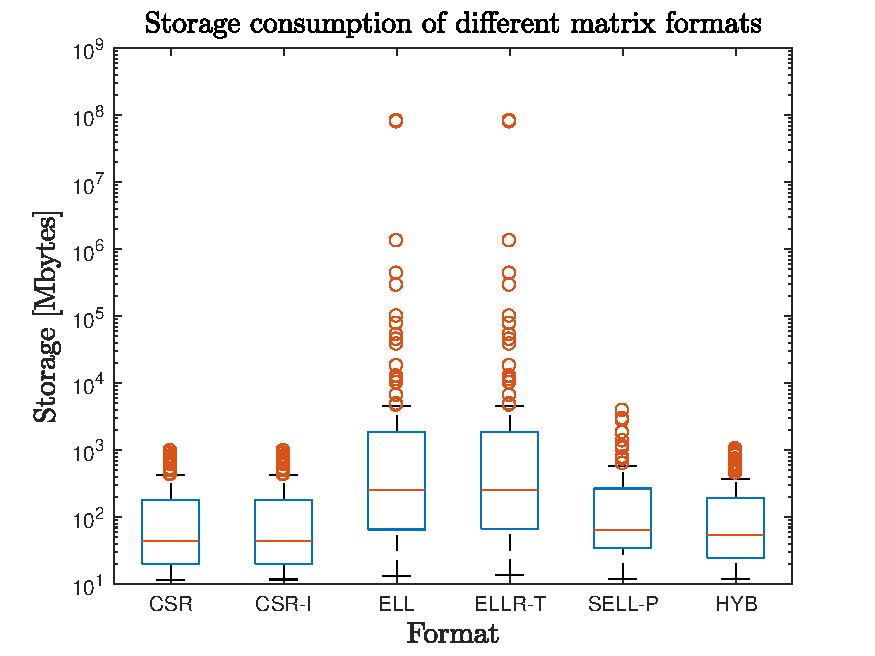
\includegraphics[width=0.48\textwidth]{plots/storage_consumption.pdf}
    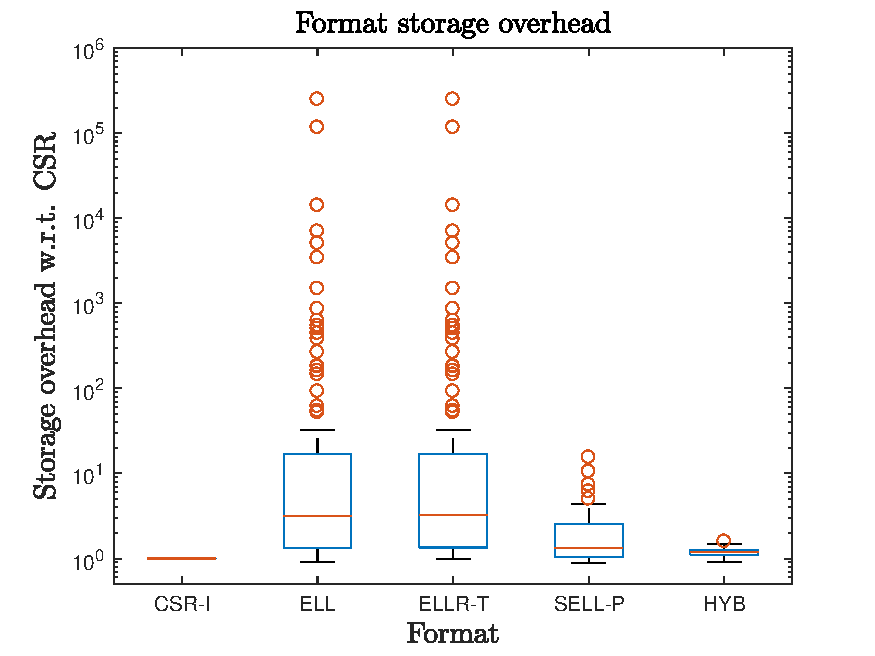
\includegraphics[width=0.48\textwidth]{plots/storage_overhead.pdf} &
\end{tabular}
\vspace*{-2ex}
    \caption{Storage consumption 
    of different sparse matrix formats (left)
    and overhead compared to CSR for these formats (right).
    The data is shown for 100 selected matrices from SMC,
    assuming $s_v$=8 (double precision) and $s_i$=4.}
\label{fig:storage}
\end{figure}

We determine the storage requirements for the CSR, ELLPACK and ELLR-T formats
from the basic properties of the matrix $A$ as:
\[
    {\cal S}_{CSR}, \quad
    {\cal S}_{ELL}     = m \cdot l_{M}(s_v + s_i), \quad \mbox{\rm and} \quad
    {\cal S}_{ELLR-T}  = \text{S}_{ELL} + m \cdot s_i,
\]
where $l_{M}$ is the number of nonzero elements in the densest matrix row.
Determining the storage requirements for the remaining two formats
is more involved.
For SELL-P we use a conversion routine from CSR to SELL-P implemented in
MAGMA-sparse and modify each memory allocation
to instead increase a counter by the amount that it was supposed to allocate.
This is not possible for HYB, as the source code is not available.
For this case, we use the \texttt{cudaMemGetInfo} routine from the
CUDA Runtime API 
to get the total amount of free device memory
before and after allocating the matrix in HYB format.
The difference between the two values is the actual storage required by HYB.
This strategy allows us to measure the storage consumption
without actually allocating the required data for all formats except HYB.
Thus, we are able to evaluate the cost even if
the problem does not fit into the GPU memory.

The experiments are carried out using a subset
of the SuiteSparse Matrix Collection (SMC).
Concretely, we first filtered the complete collection (2,757 problem instances)
keeping only real-valued instances with $10^6 \leq n_z < 10^8$ (491 problems),
and then randomly selected 100 cases%
\footnote{The list of cases employed in the experiments can be downloaded from
\mbox{\url{http://www3.uji.es/~flegar/2017_csri/matrices.txt}}.}
among these
(about 20\% of the filtered problems and 3.6\% of the complete collection). 
The limits for $n_z$ were chosen to allow the utilization
of the full processing potential of GPUs,
while keeping the storage requirements low enough
to fit the matrix into the GPU memory.
We believe this is a representative subset of the
problems for which a GPU accelerator can be beneficial,
not being biassed to any particular format.

\begin{figure}[t]
\begin{tabular}{c}
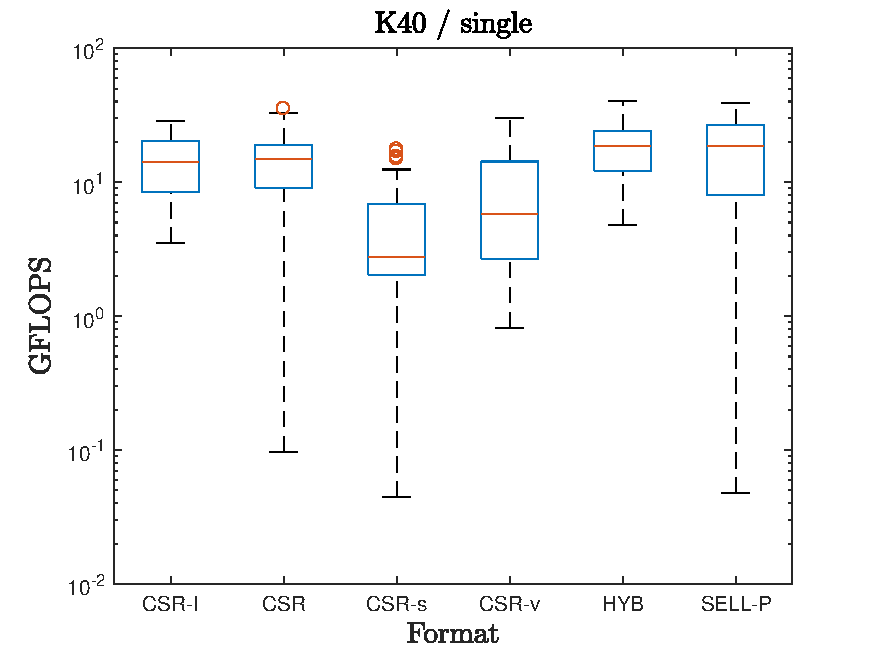
\includegraphics[width=0.48\textwidth]{plots/range_K40_single.pdf}
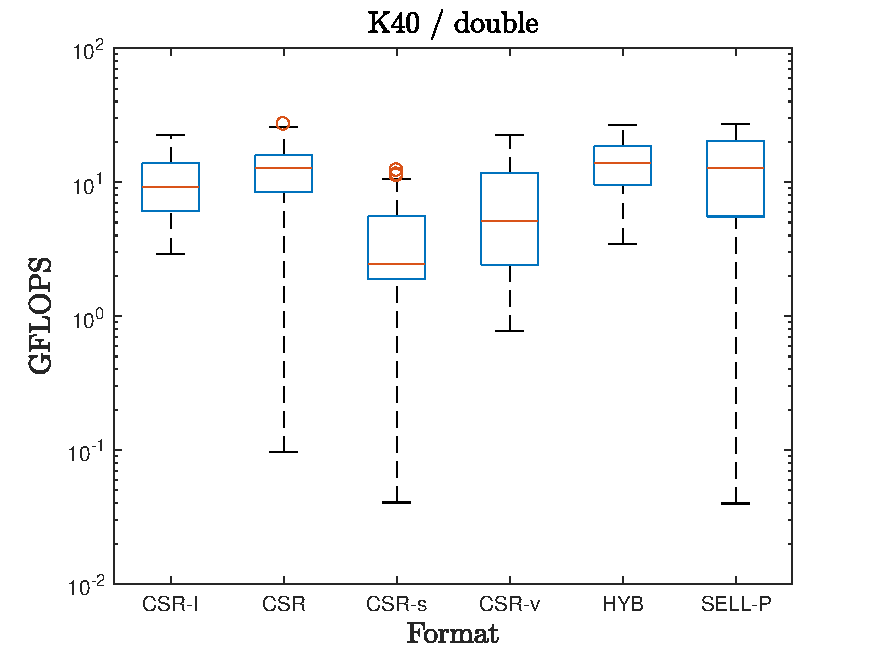
\includegraphics[width=0.48\textwidth]{plots/range_K40_double.pdf}\\
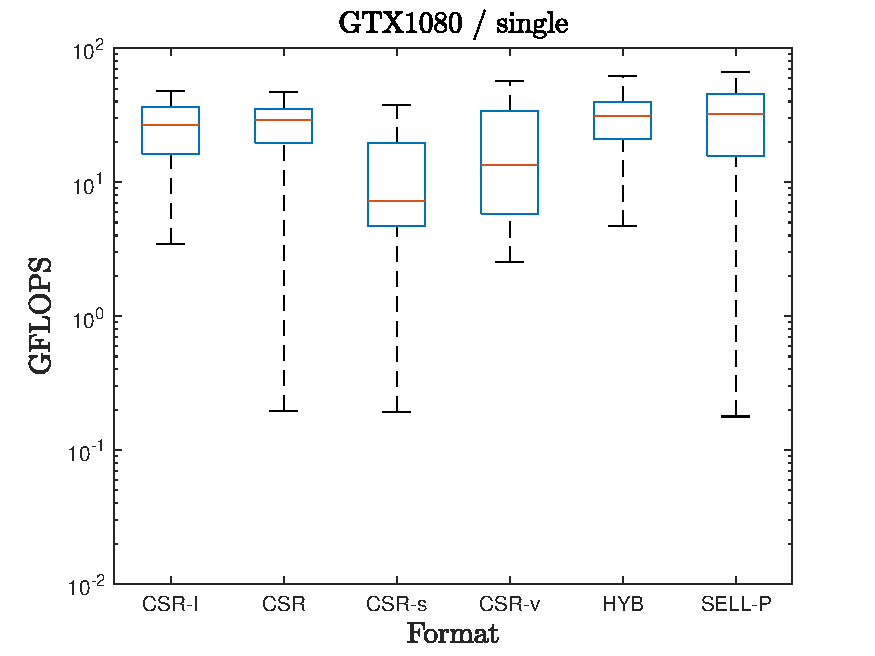
\includegraphics[width=0.48\textwidth]{plots/range_GTX1080_single.pdf}
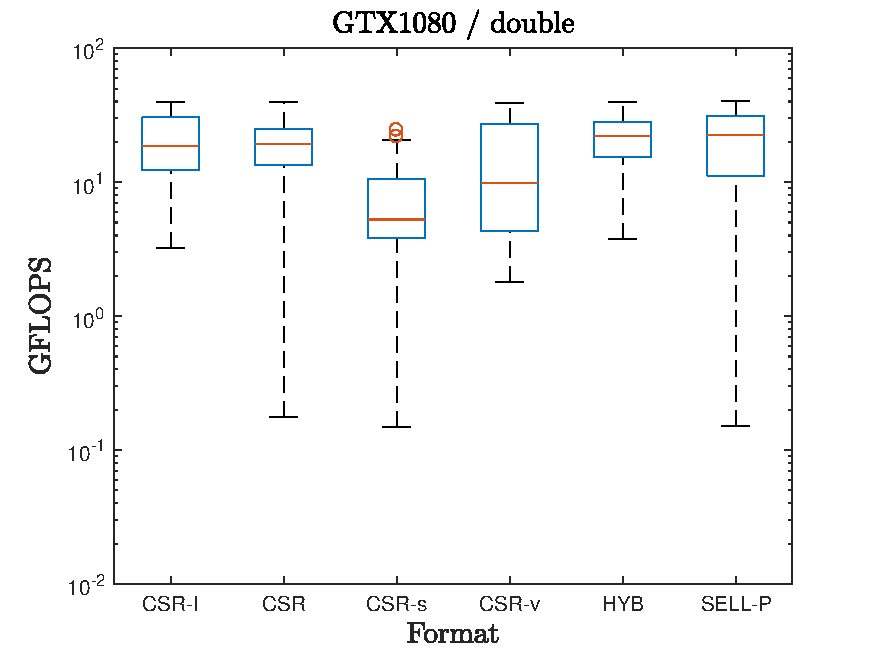
\includegraphics[width=0.48\textwidth]{plots/range_GTX1080_double.pdf}
\end{tabular}
\vspace*{-2ex}
\caption{GFLOPS distribution of \spmv implementations on K40 (top)
    and GTX1080 (bottom), using SP and DP arithmetic (left and right, respectively).}
\label{fig:distribution}
\end{figure}

\subsection{Memory consumption}

We commence our evaluation with an analysis of storage consumption
of different matrix formats for the 100 selected matrices from SMC.
Figure~\ref{fig:storage} shows that,
for most cases, CSR is the format that requires the lowest amount of memory,
and the additional storage required to save the \srow array in \bcsr
is negligible.
HYB requires some additional memory,
but this is still within a limit
of 2$\times$ compared with CSR.
SELL-P performs quite poorly for some cases,
consuming up to 11$\times$ more memory than CSR;
while ELLPACK and ELLR-T consume even up to 5 orders of magnitude more
storage space in some cases.
As a result, even though the storage required by CSR and HYB is under 1~Gbyte
for all selected problems, the storage requirements can grow to 3~Gbytes for SELL-P
and even to 100~Tbytes for ELLPACK and ELLR-T.
This shows that the last two layouts cannot be considered as general formats.
Since the focus of this work is on \spmv algorithms
for general matrices,
possibly with an irregular nonzero distribution,
we omit ELLPACK and ELLR-T from the following experiments.

\begin{figure}[t]
\begin{tabular}{c}
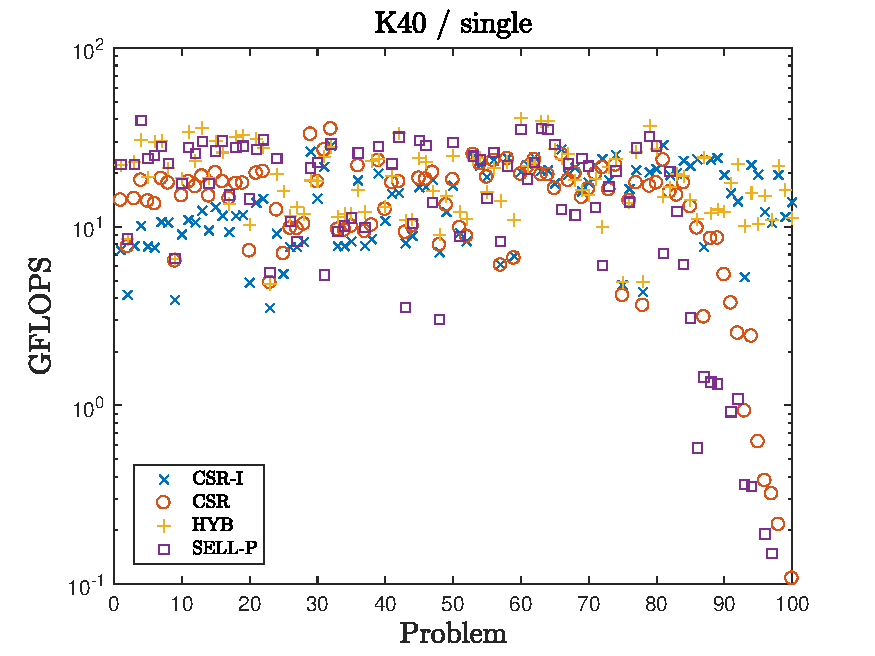
\includegraphics[width=0.48\textwidth]{plots/performance_K40_single.pdf}
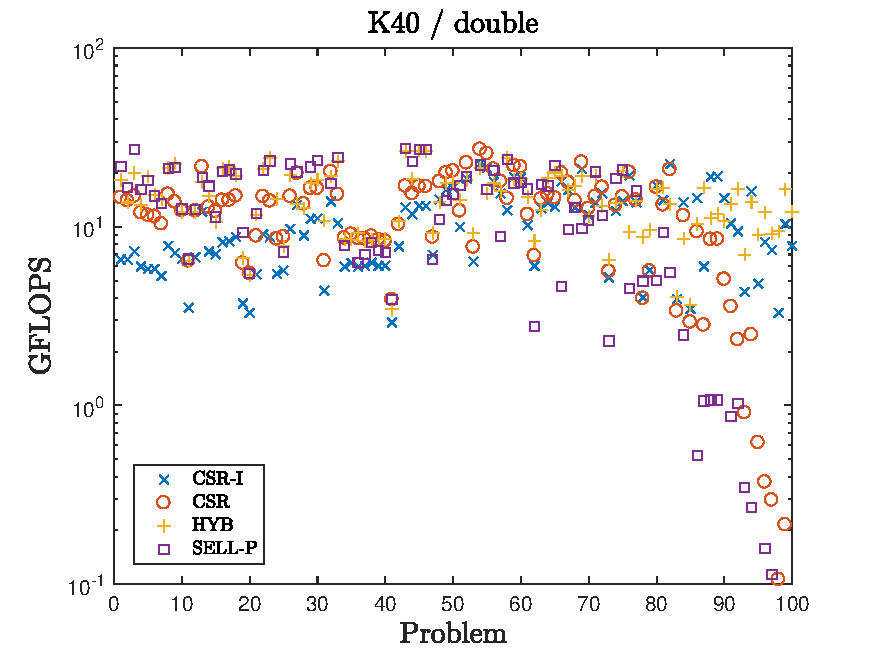
\includegraphics[width=0.48\textwidth]{plots/performance_K40_double.pdf}\\
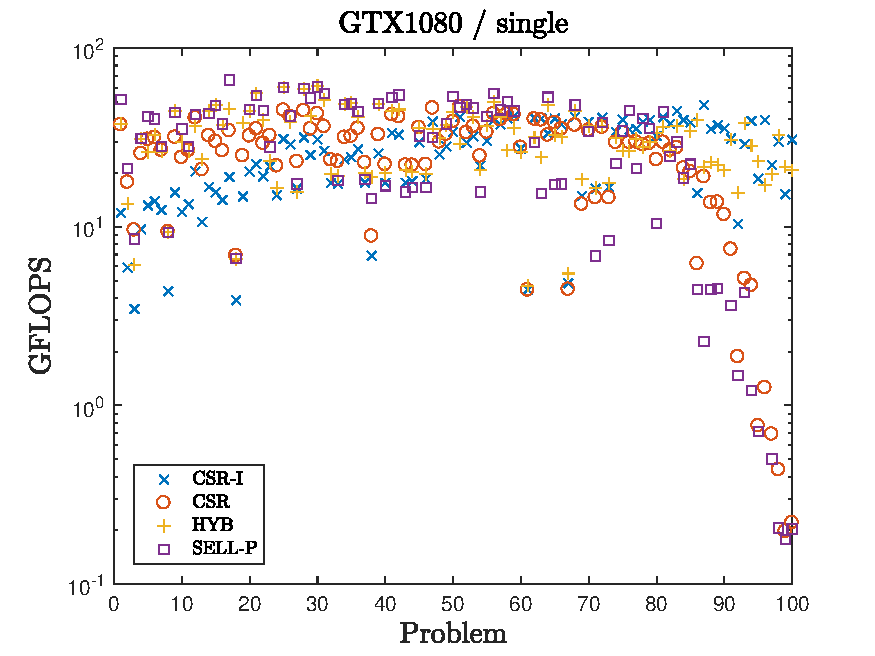
\includegraphics[width=0.48\textwidth]{plots/performance_GTX1080_single.pdf}
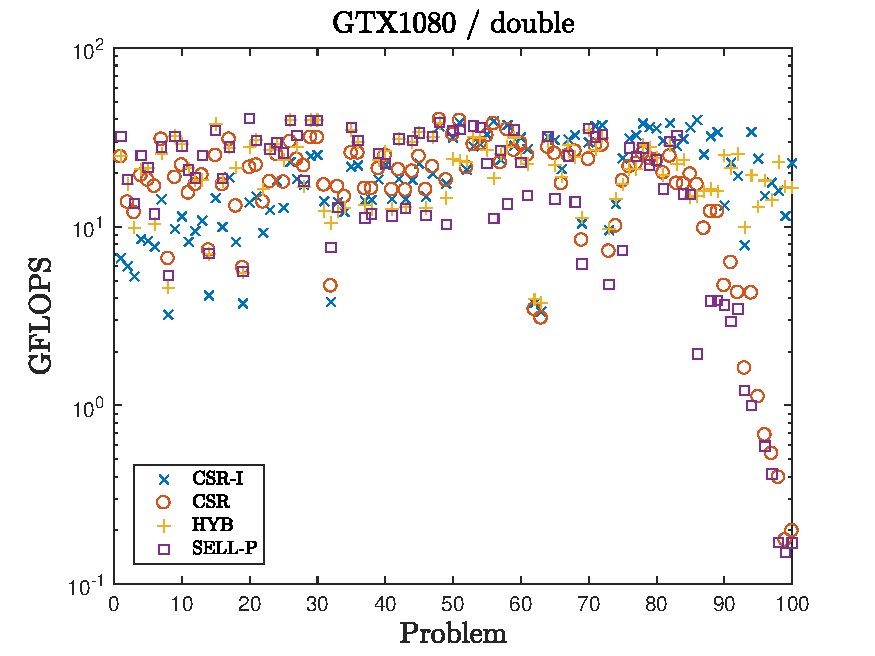
\includegraphics[width=0.48\textwidth]{plots/performance_GTX1080_double.pdf}
\end{tabular}
\vspace*{-2ex}
\caption{Comparison of \spmv implementations on K40 (top)
    and GTX1080 (bottom), using SP and DP arithmetic (left and right, respectively).}
\label{fig:performance}
\end{figure}

\subsection{Global comparison}

The results in Figure~\ref{fig:distribution}
show the distribution of the GFLOPS rates
by means of ``box-and-whisker'' plots.
This experiment reveals that
the median GFLOPS rate for our \bcsr format
(red line inside the blue boxes) is similar 
to those of the specialized kernel for CSR in cuSPARSE, HYB and SELL-P;
and all four present considerably higher
GFLOPS medians than those observed for CSR-s and CSR-v.
For this reason, we omit CSR-s and CSR-v from further discussion.
Furthermore, the lower ``whisker'' attached to the boxes in
Figure~\ref{fig:distribution},
which comprises the first quartile (i.e. 25\%) of the cases,
show that both CSR and SELL-P encounter a
considerable number of ``ill-conditioned'' cases
from the point of view of performance,
delivering notably lower GFLOPS rates for those.
In contrast, \bcsr and HYB feature a more consistent performance rate.
This behaviour can also be observed in Figure~\ref{fig:performance}.
(The problem instances in this figure are ordered
by speed-up/slow-down of \bcsr over cuSPARSE CSR.)
For regular cases, appearing in the left-hand side of the plots, \bcsr is outperformed
by all implementations due to its higher arithmetic intensity
and use of atomic operations.
In contrast, for irregular problems, in the right-hand side of the plots,
the only implementation that matches its performance is HYB,
which, in addition to higher storage consumption,
is not suitable for other types of operations.
We do not evaluate the cost of transformation
from CSR to the other formats included in our experiments.
For \bcsr, as discussed in the previous section, this cost is small,
or even negligible if this transformation is overlapped
with the first transfer of the matrix data to the GPU memory.

\begin{figure}[t]
\begin{tabular}{c}
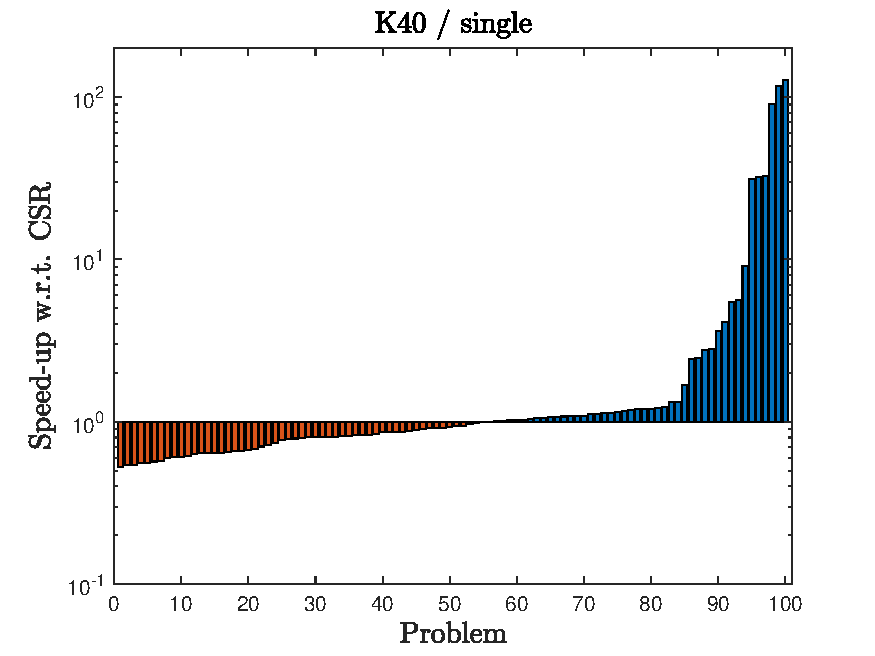
\includegraphics[width=0.48\textwidth]{plots/speedup_K40_single.pdf}
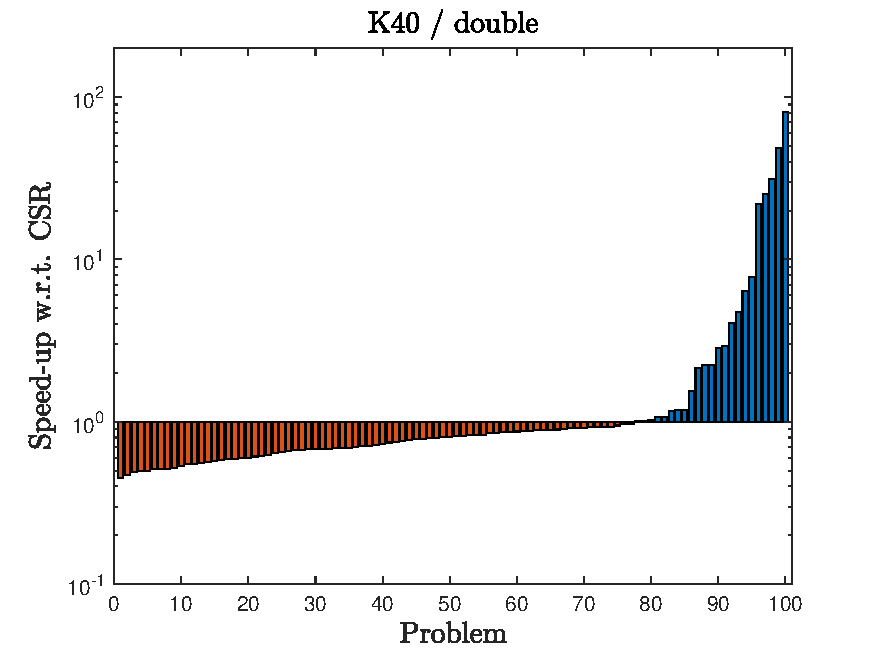
\includegraphics[width=0.48\textwidth]{plots/speedup_K40_double.pdf}\\
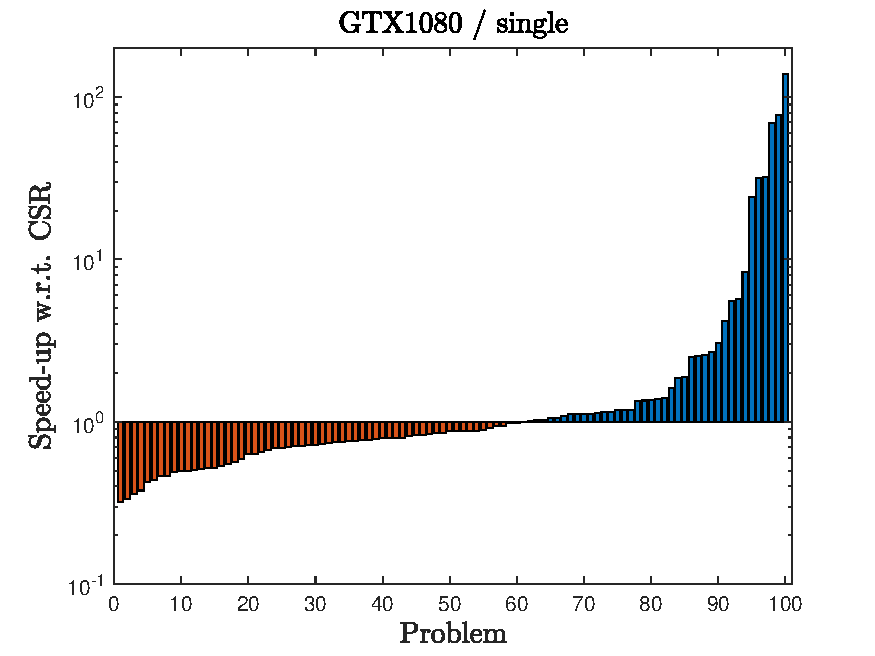
\includegraphics[width=0.48\textwidth]{plots/speedup_GTX1080_single.pdf}
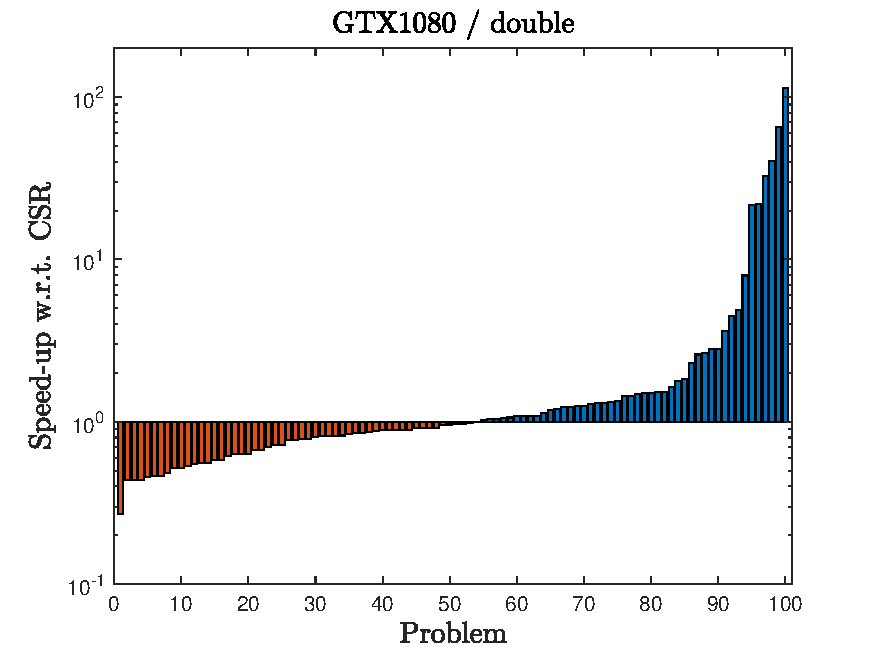
\includegraphics[width=0.48\textwidth]{plots/speedup_GTX1080_double.pdf}
\end{tabular}
\vspace*{-2ex}
\caption{Comparison between CSR and \bcsr implementations of \spmv on K40 (top) and GTX1080 (bottom), using SP and DP arithmetic (left and right, respectively).}
\label{fig:bcsr}
\end{figure}

\subsection{Detailed comparison of CSR and \bcsr.}
As argued at the beginning of this paper,
the specific goal for our \bcsr variant
is to ensure an efficient execution of \spmv
when the matrix exhibits an irregular row distribution of its nonzero entries,
while maintaining the data layout of the regular version of CSR
(and roughly its memory requirements).
To close the experiments, we evaluate the performance of these two formats in more detail.
Figure~\ref{fig:bcsr} illustrates the throughput of
the \bcsr variant with respect to that of CSR from cuSPARSE
for each problem instance.
In these plots, we employ a logarithmic scale for the $y$-axis,
and the problems instances are sequenced in the
$x$-axis in increasing order of difference in favour of \bcsr.
For three of the configurations: K40-SP and GTX 1080-SP/DP,
\bcsr outperforms CSR in about 40--50\% of the problems,
and the difference in favour of the former
comes in a factor that can raise more than 100$\times$.
Compared with this, the highest loss of \bcsr
shows a factor that is at most 0.3$\times$.
For  K40-DP
\bcsr is superior for 24\% of the problem instances.
This is explained by the lack of hardware support for DP atomic updates in this architecture.

\begin{figure}[t]
\begin{tabular}{cc}
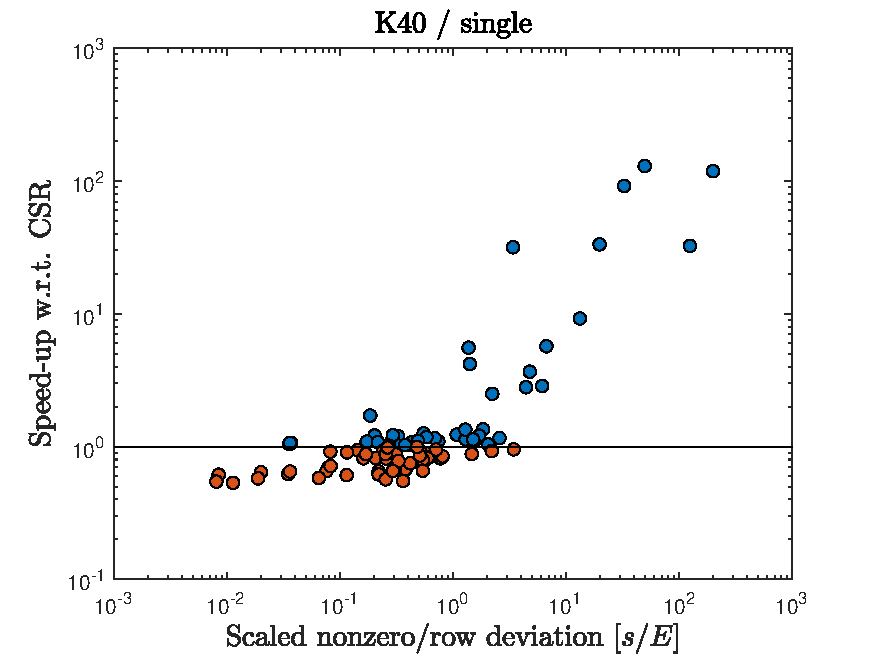
\includegraphics[width=0.48\textwidth]{plots/std_speedup_K40_single.pdf} &
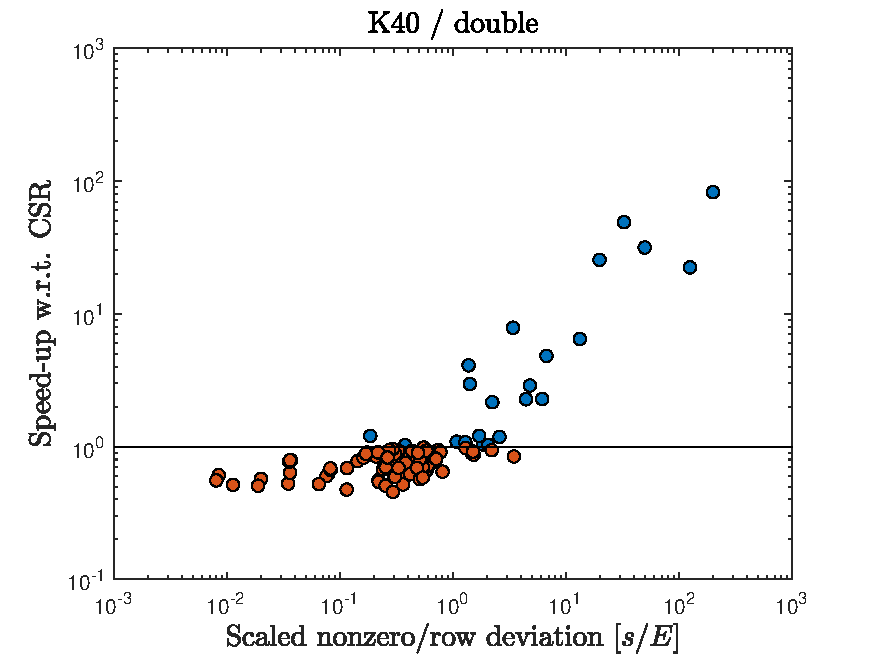
\includegraphics[width=0.48\textwidth]{plots/std_speedup_K40_double.pdf}\\
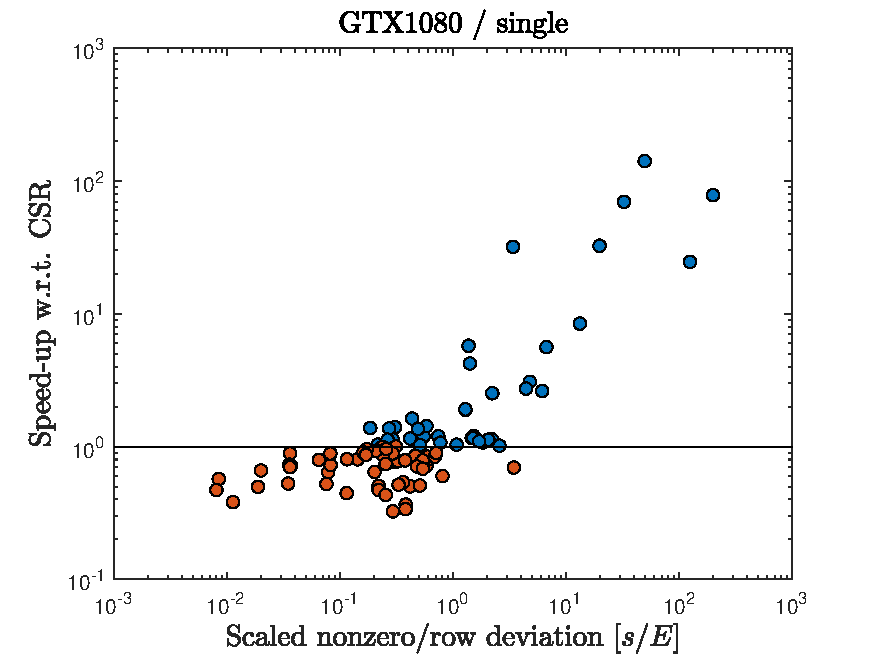
\includegraphics[width=0.48\textwidth]{plots/std_speedup_GTX1080_single.pdf} &
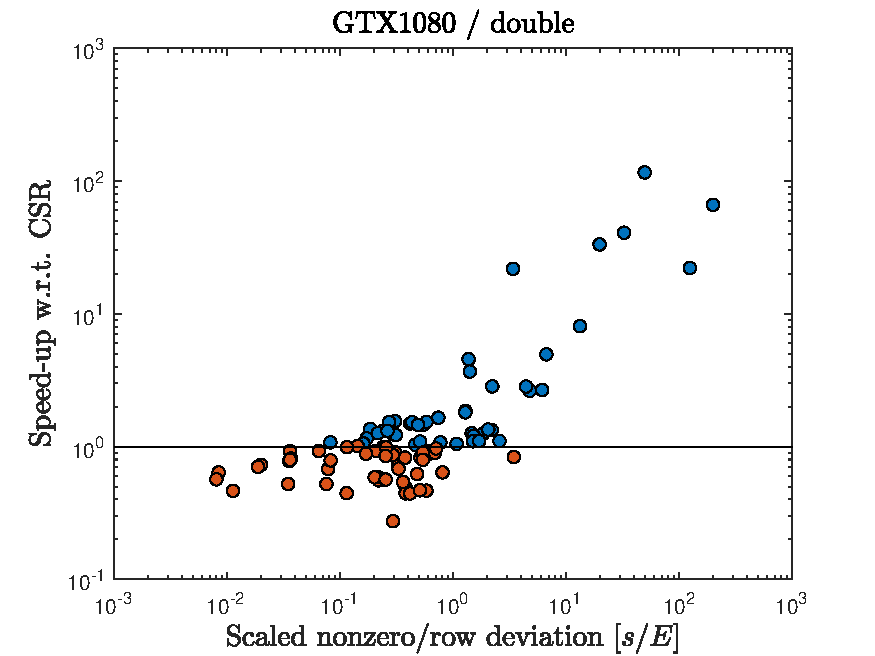
\includegraphics[width=0.48\textwidth]{plots/std_speedup_GTX1080_double.pdf}
\end{tabular}
\vspace*{-2ex}
\caption{Relationship between $s[n_{zr}]/E[n_{zr}]$ ($x$-axis)
    and speed-up/slow-down of \bcsr over CSR ($y$-axis)
    on K40 (top) and GTX1080 (bottom)
    using SP and DP arithmetic (left and right, respectively).}
\label{fig:deviation}
\end{figure}

Even though \bcsr shows notable acceleration over CSR
for a fair fraction of the problem instances,
an optimal hybrid strategy is obtained if \bcsr is applied to compute \spmv
for matrices in this subset only,
while the operation relies on CSR for the remaining cases.
Note that this is possible because \bcsr maintains the same structure as CSR,
with just an additional vector to store the starting rows of each segment.
In contrast, an attempt to combine CSR with any
of the other GPU-specialized formats (HYB, SELL-P, ELLPACK, ELLR-T)
would incur a considerable increase in the amount
of stored information (even a complete duplication).
Still, a relevant question is whether we can choose {\em a priori}
to rely on either CSR or \bcsr for a particular \spmv.
Figure~\ref{fig:deviation} shows that this is indeed the case
if we have a rough statistical estimation
of the distribution of the number of nonzero entries per row $n_{zr}$.
Concretely, the figure depicts the relationship
between the performance of \bcsr over CSR
and the standard deviation-to-mean ratio:
$s[n_{zr}]/E[n_{zr}]$.
The plots in the figure show a clear separation at
$s[n_{zr}]/E[n_{zr}]$=1 for both architectures and precisions.
For ratios grater than one, \bcsr is slightly slower for only one test matrix
and shows a significant acceleration for the rest of the cases on GTX1080.
The K40 GPU exhibits a similar behaviour,
with only several cases slightly slower and the majority
achieving significantly higher performance for ratios above this threshold.
For ratios between 0.1 and 1, the faster algorithm
depends on the matrix, but the majority of cases favour cuSPARSE CSR.
For extremely regular sparsity patterns, with ratios below 0.1,
cuSPARSE CSR is the clear winner.
